\section{User Interface Prototype}

\begin{figure}[!h]
    \begin{minipage}{0.3\textwidth}
        \centering
        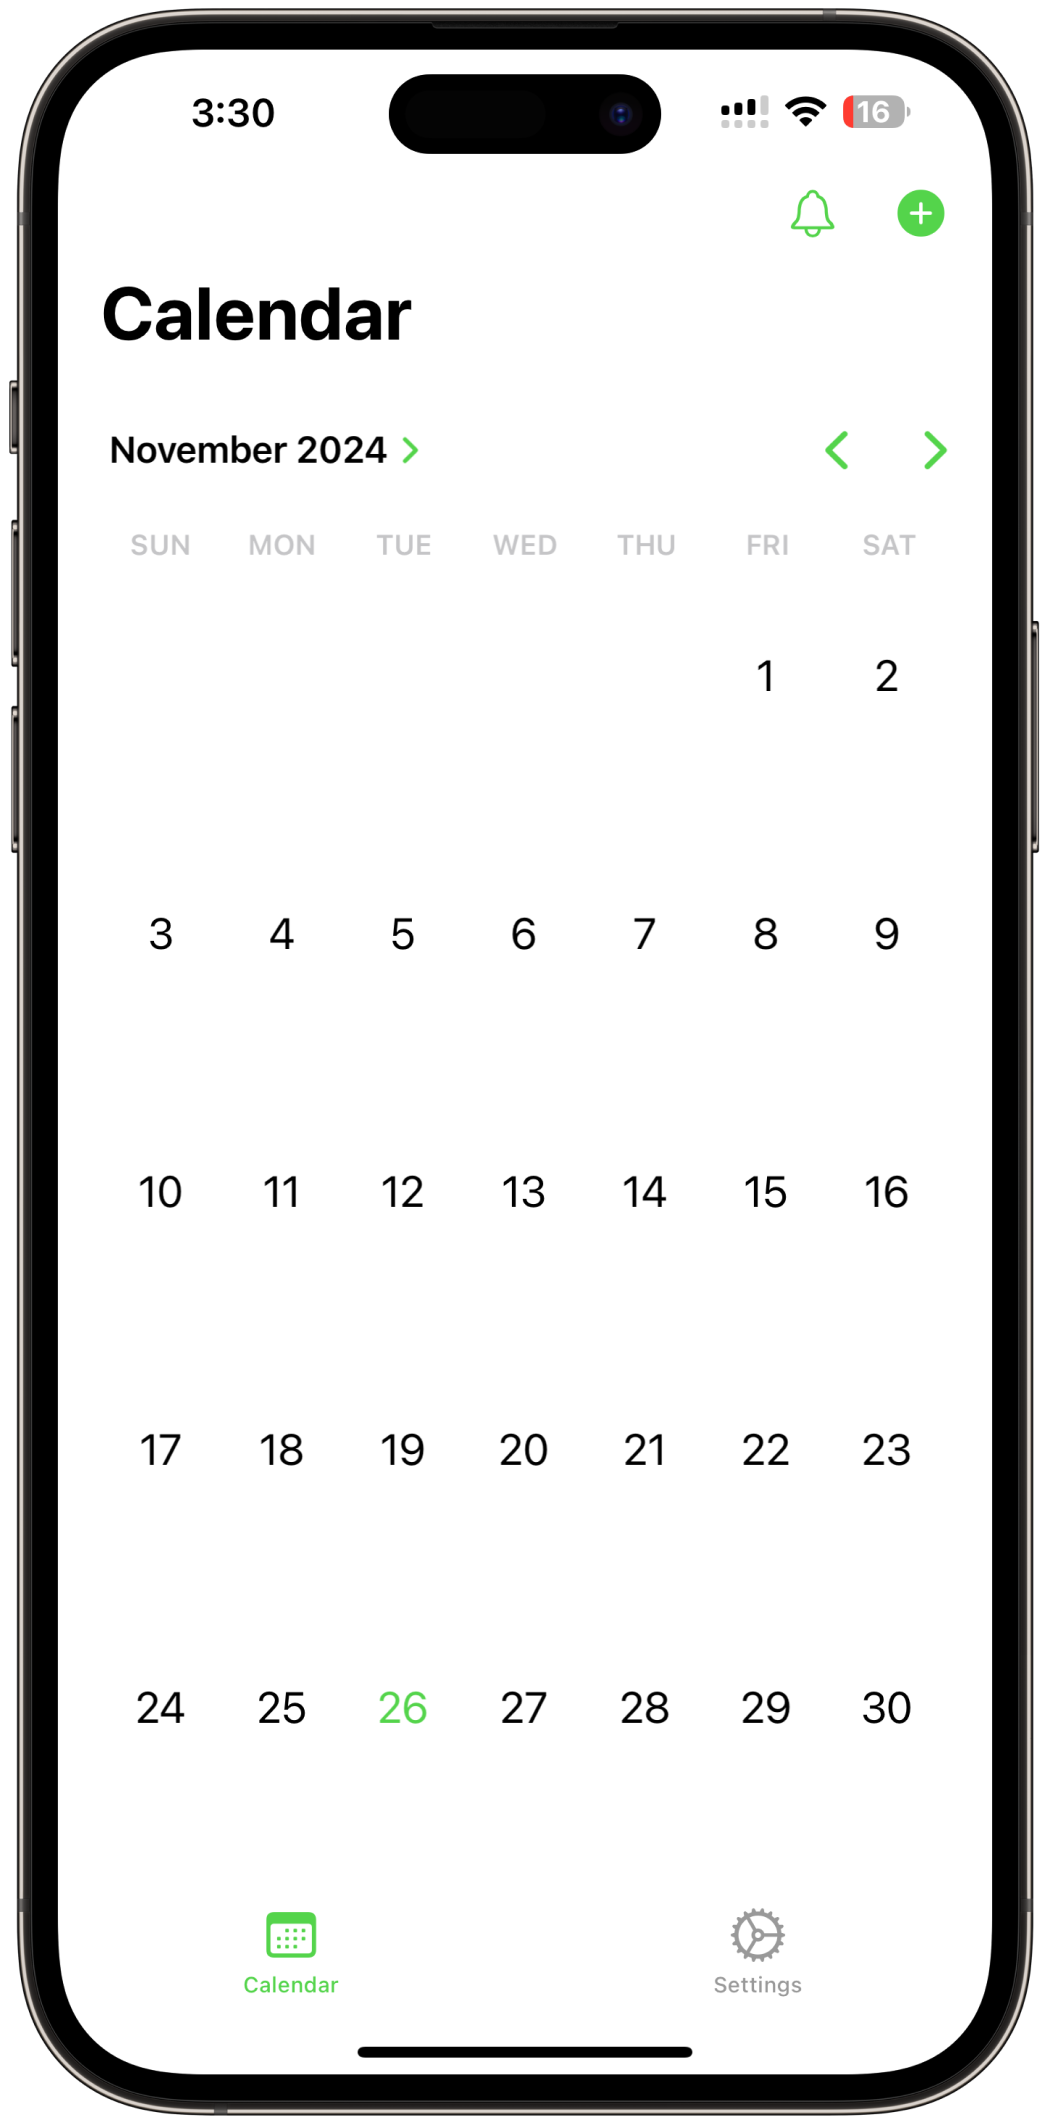
\includegraphics[width=\textwidth]{images/screen1.png}
        \caption{UI Screen 1: Onboarding View}
        \label{fig:ui-screen-1}
    \end{minipage}
    \hfill
    \begin{minipage}{0.65\textwidth}
        In Figure \ref{fig:ui-screen-1}, the screen shows the user the steps he needs to take in the future so he knows what he is going to do. It also has two way of authenticating, Google and Email (Magic Link).
    \end{minipage}
\end{figure}

\begin{figure}[!h]
    \begin{minipage}{0.65\textwidth}
        In Figure \ref{fig:ui-screen-2}, users can click on the text that shows the currently selected month, in this case ``November 2024'' and get a selector wheel that allows them to choose a month and a year to navigate to.
    \end{minipage}
    \hfill
    \begin{minipage}{0.3\textwidth}
        \centering
        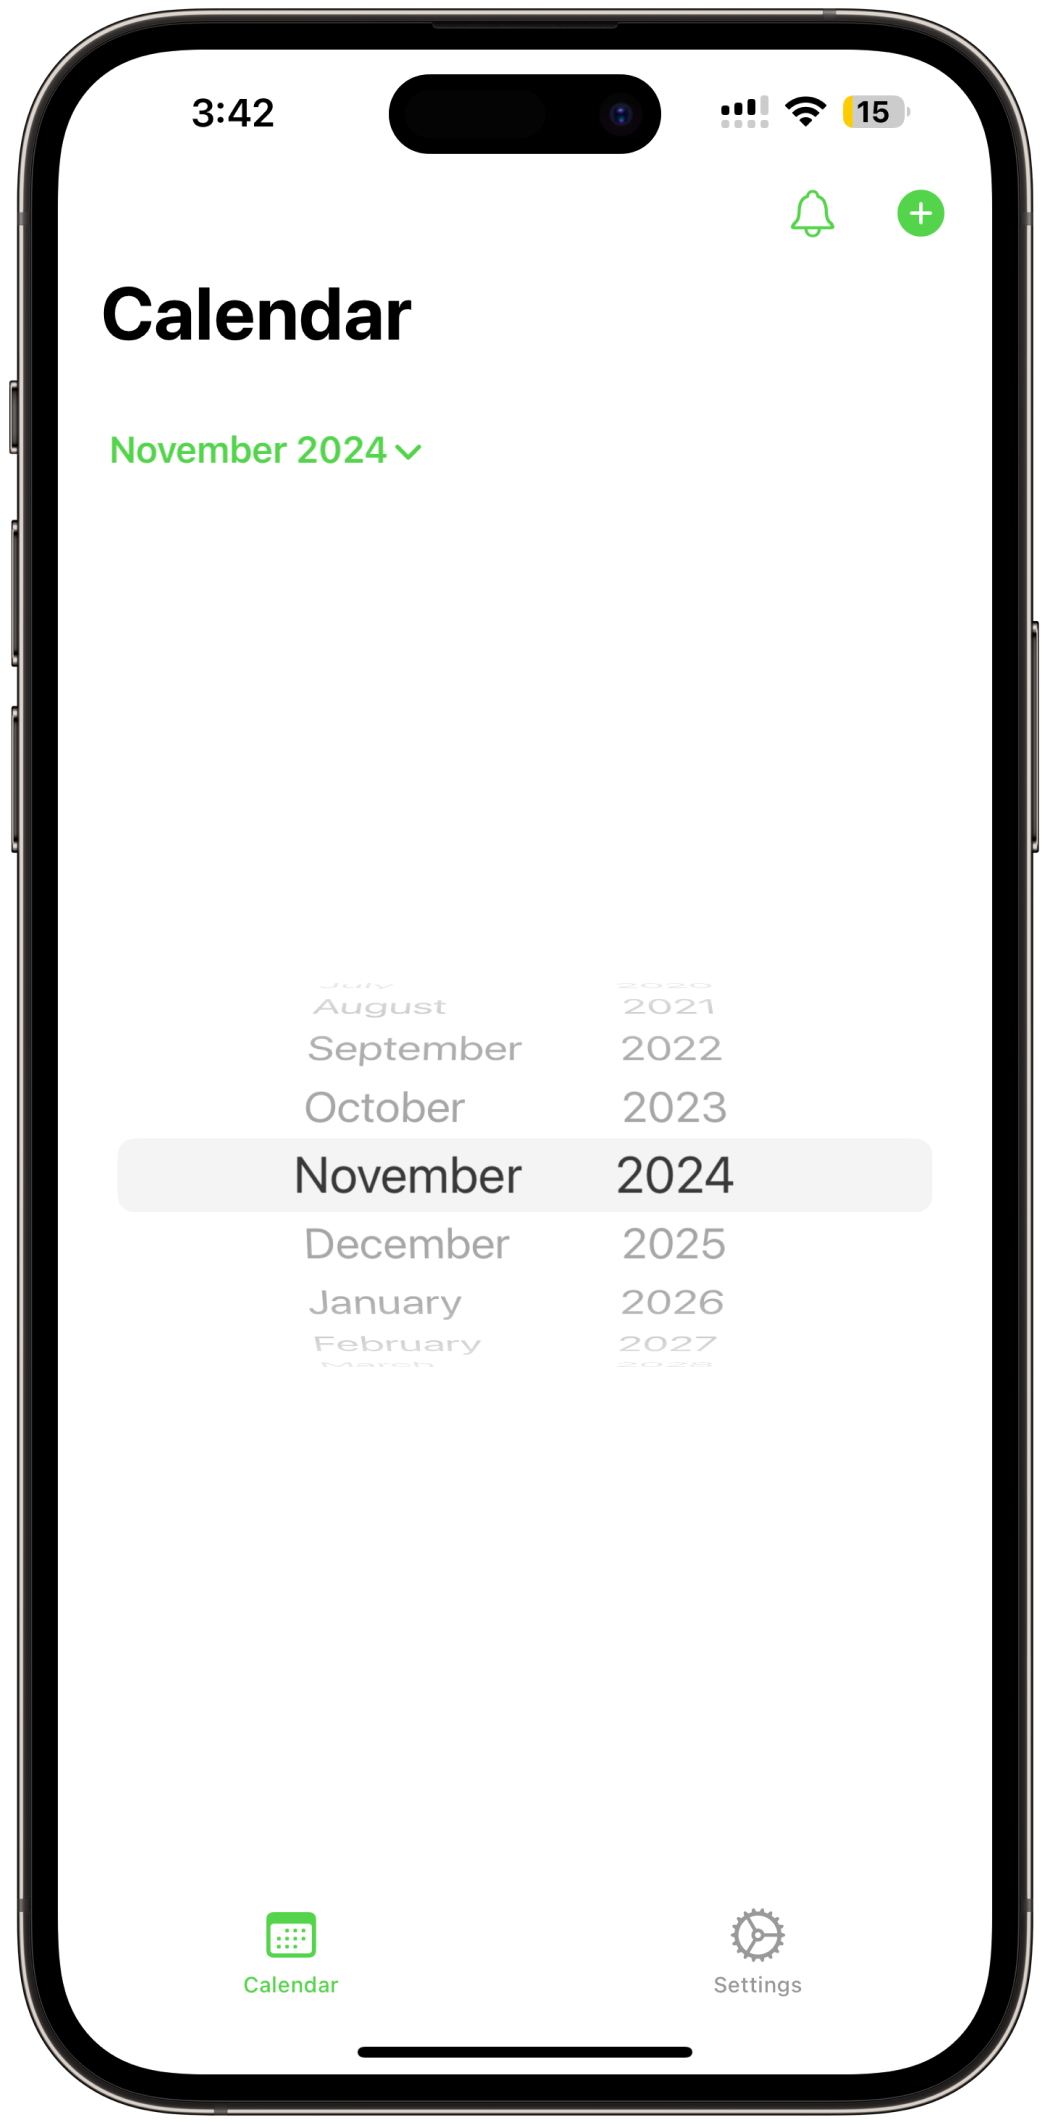
\includegraphics[width=\textwidth]{images/screen2.png}
        \caption{UI Screen 2: Month \& Year Selector}
        \label{fig:ui-screen-2}
    \end{minipage}
\end{figure}

\begin{figure}[!h]
    \begin{minipage}{0.3\textwidth}
        \centering
        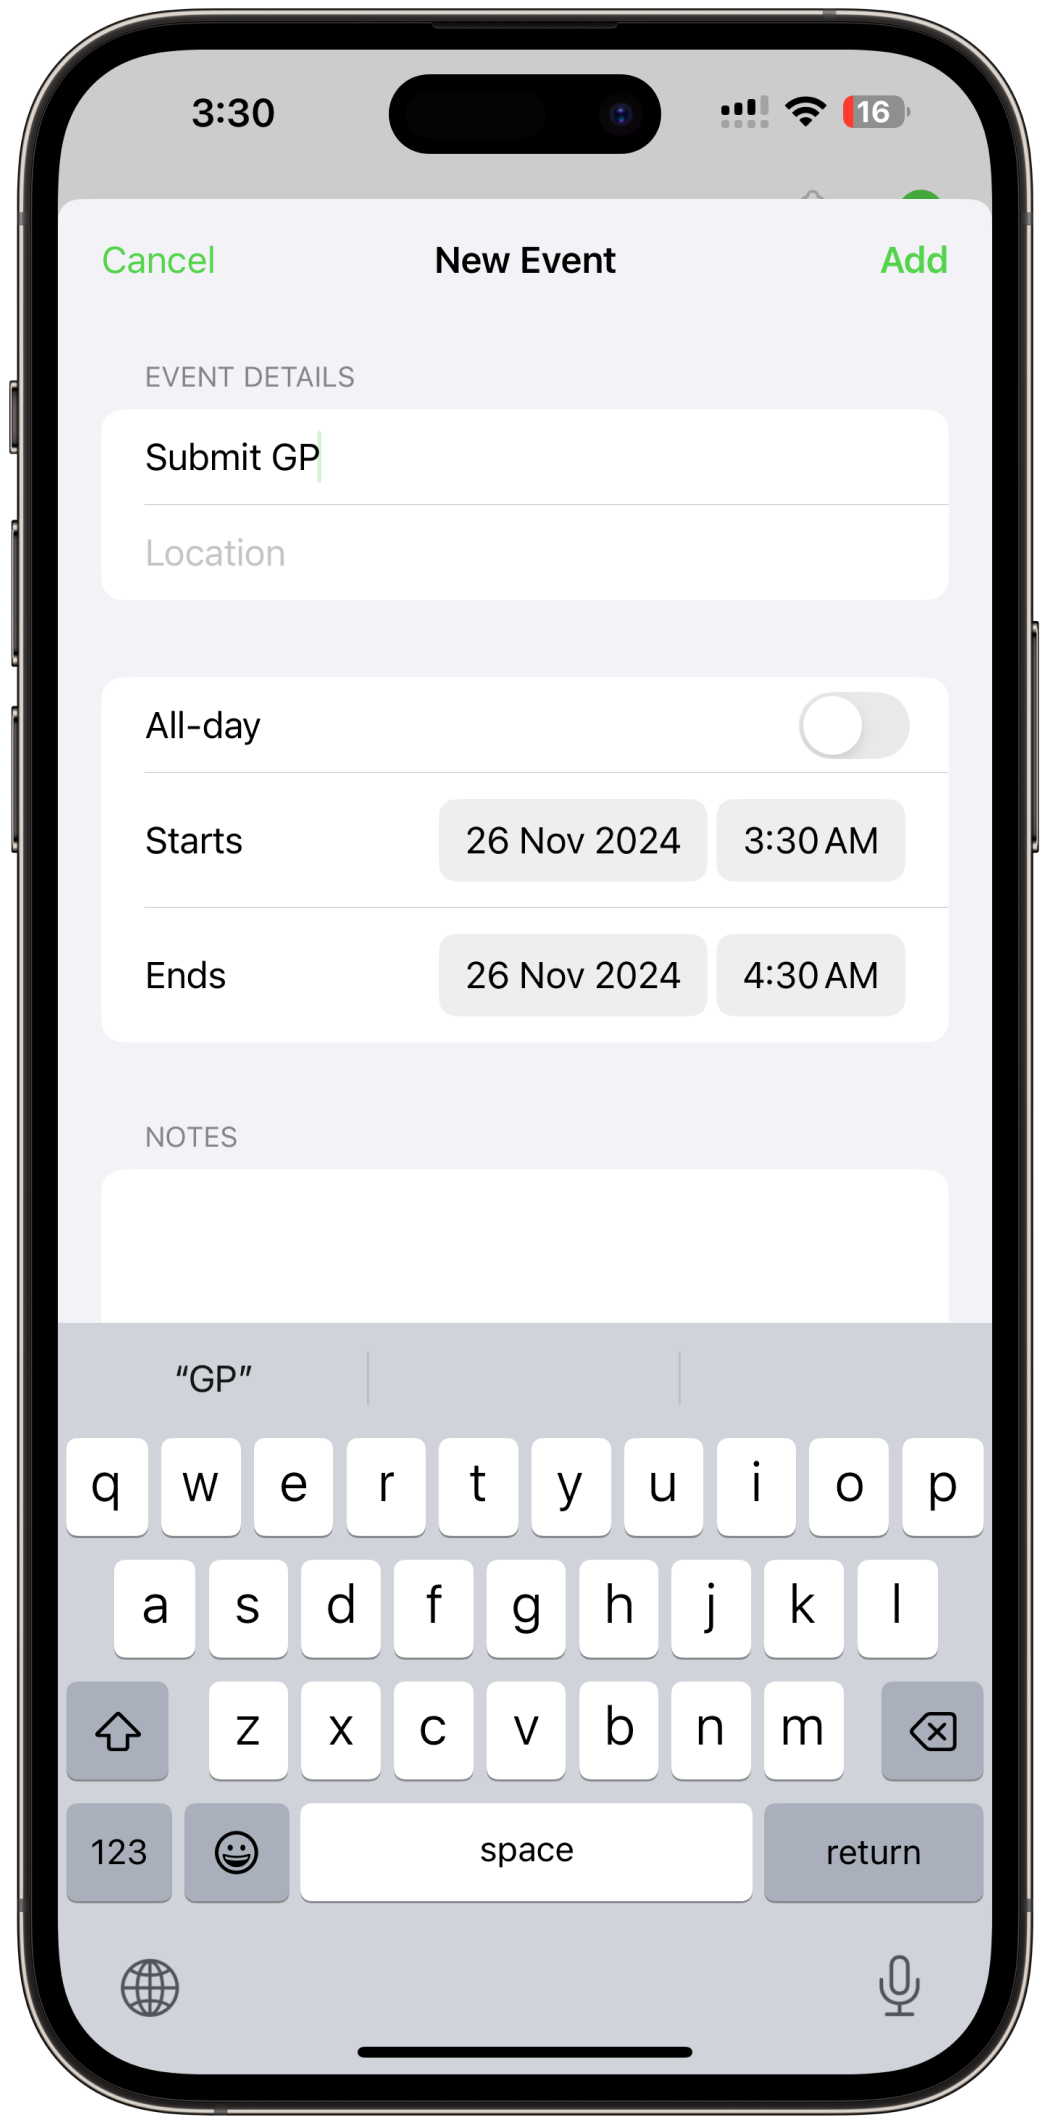
\includegraphics[width=\textwidth]{images/screen3.png}
        \caption{UI Screen 3: Add Event View - Default}
        \label{fig:ui-screen-3}
    \end{minipage}
    \hfill
    \begin{minipage}{0.65\textwidth}
        Your explanation for Screen 3 goes here. This text will appear to the right 
        of the third screenshot. You can describe the final state of the interface 
        and what the user can accomplish on this screen.
    \end{minipage}
\end{figure}

\begin{figure}[!h]
    \begin{minipage}{0.65\textwidth}
        In Figure \ref{fig:ui-screen-4}, the calendar view represents the user's schedule. It shows upcoming events, past events, and current events. It also has two buttons at the top, notifications and add event buttons. Users can swipe left and right to navigate months. The current day is colored in green.
    \end{minipage}
    \hfill
    \begin{minipage}{0.3\textwidth}
        \centering
        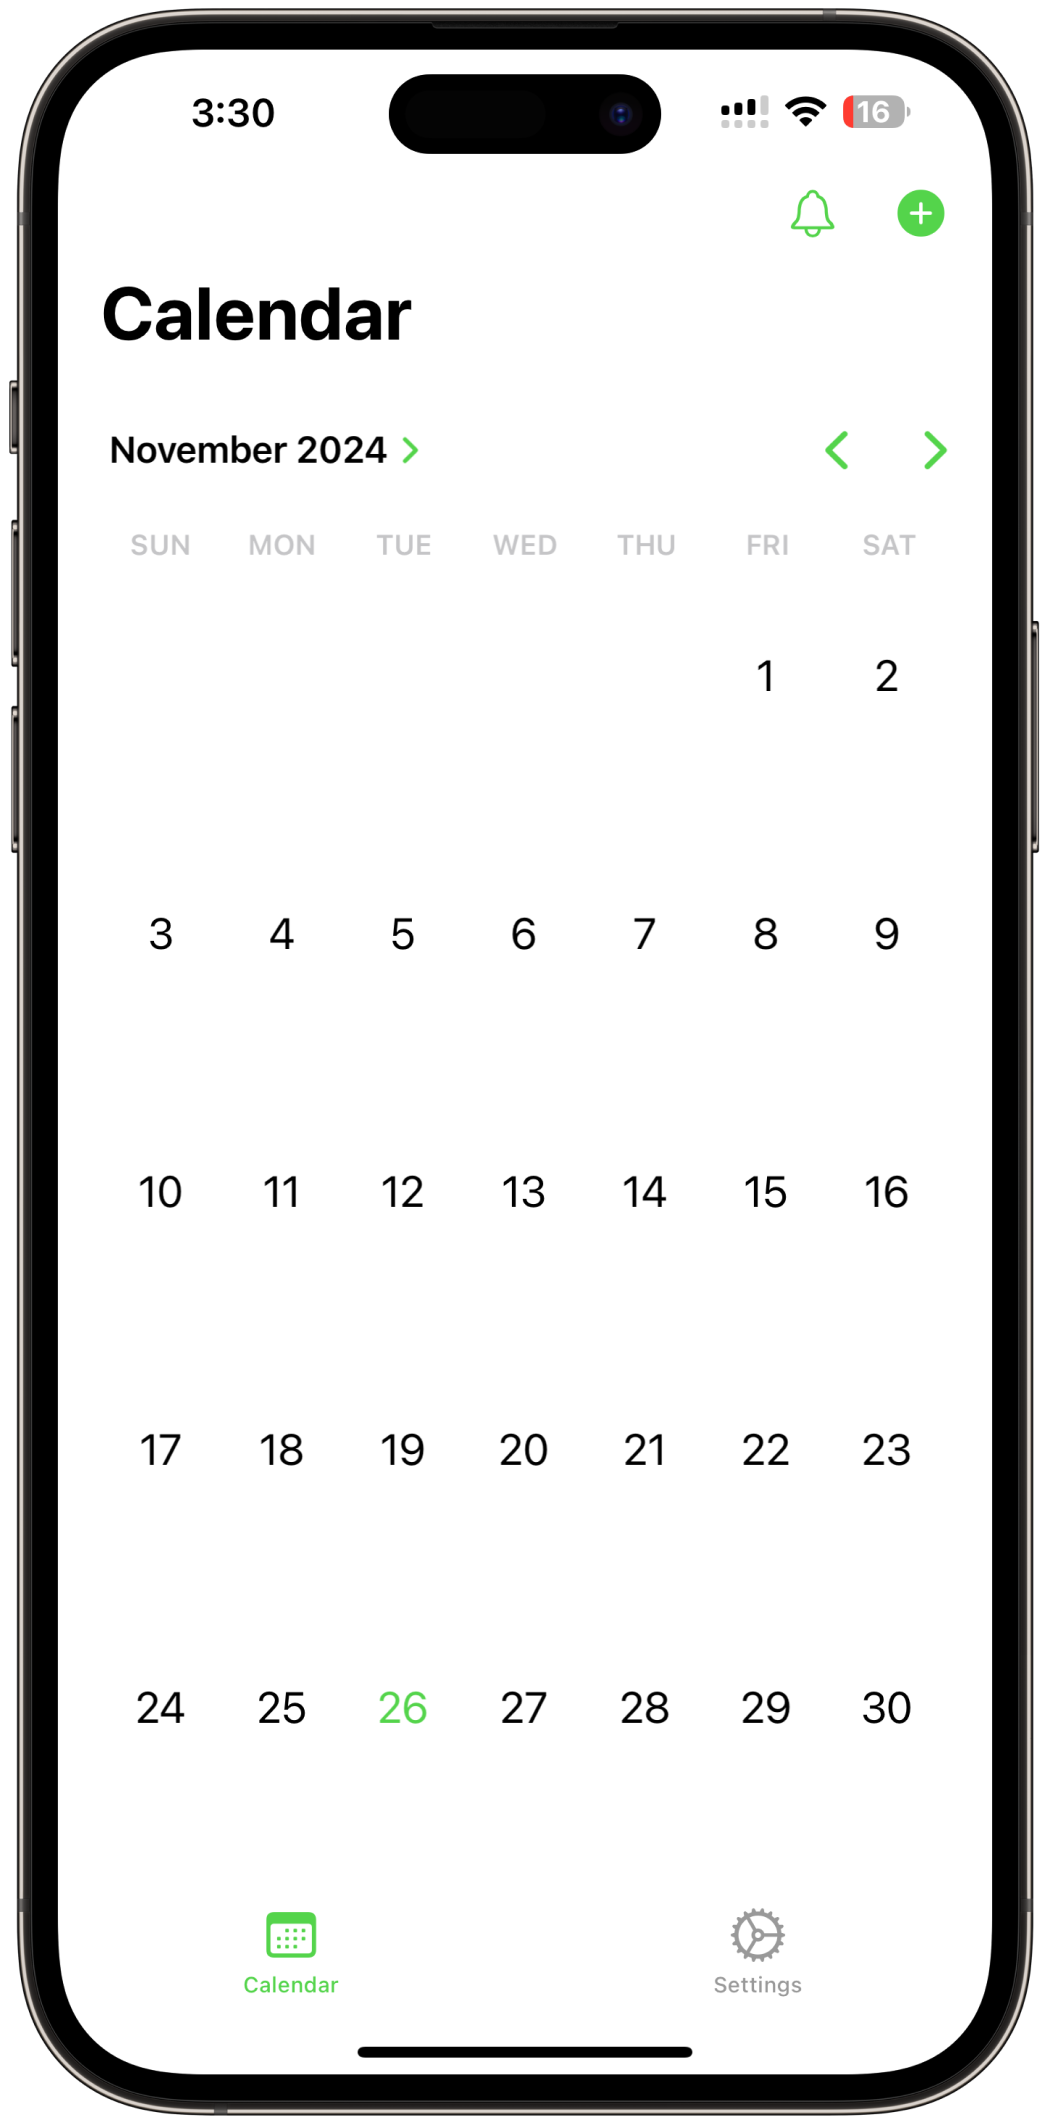
\includegraphics[width=\textwidth]{images/screen4.png}
        \caption{UI Screen 4: Calendar View}
        \label{fig:ui-screen-4}
    \end{minipage}
\end{figure}

\begin{figure}[!h]
    \begin{minipage}{0.3\textwidth}
        \centering
        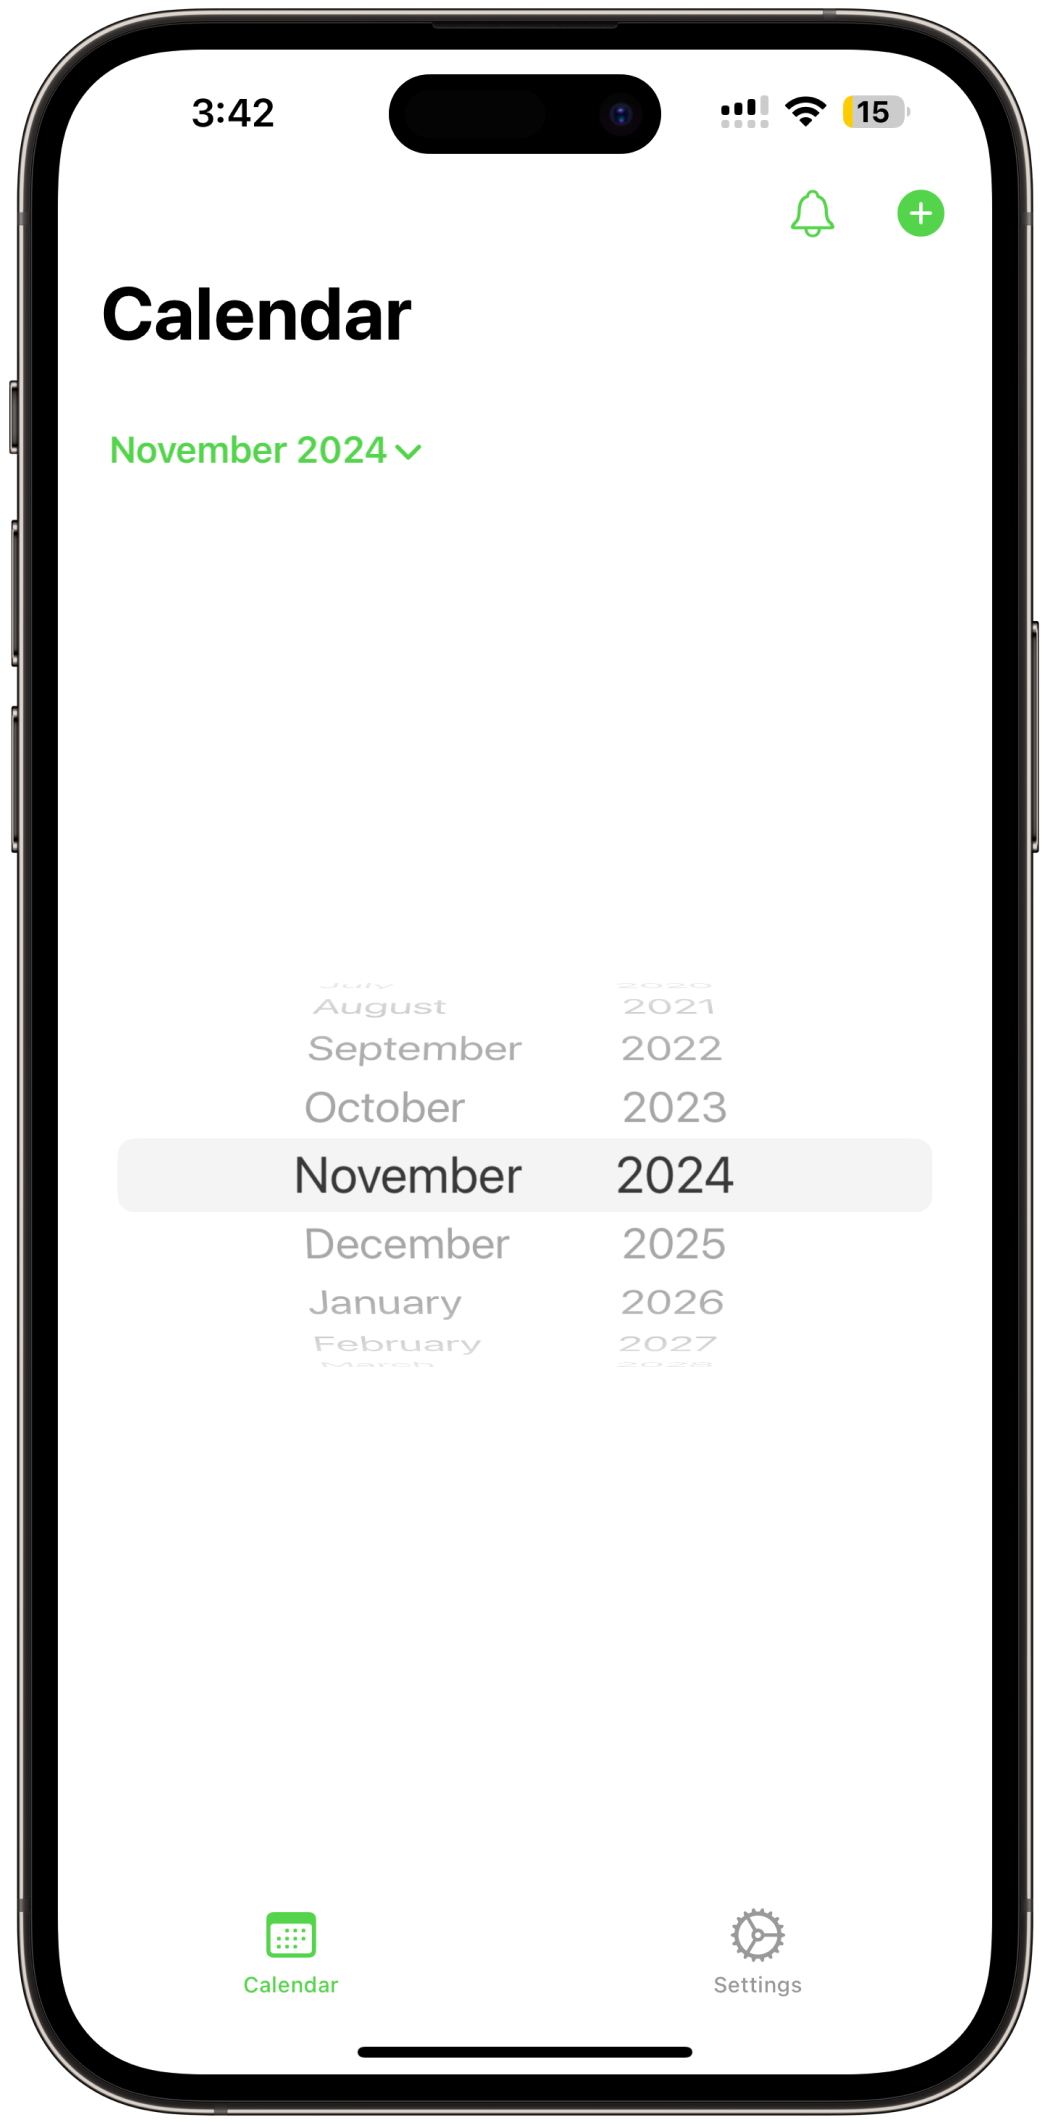
\includegraphics[width=\textwidth]{images/screen5.png}
        \caption{UI Screen 5: Add Event View - Time Selector}
        \label{fig:ui-screen-5}
    \end{minipage}
    \hfill
    \begin{minipage}{0.65\textwidth}
        Your explanation for Screen 3 goes here. This text will appear to the right 
        of the third screenshot. You can describe the final state of the interface 
        and what the user can accomplish on this screen.
    \end{minipage}
\end{figure}

\begin{figure}[!h]
    \begin{minipage}{0.65\textwidth}
        Your explanation for Screen 3 goes here. This text will appear to the right 
        of the third screenshot. You can describe the final state of the interface 
        and what the user can accomplish on this screen.
    \end{minipage}
    \hfill
    \begin{minipage}{0.3\textwidth}
        \centering
        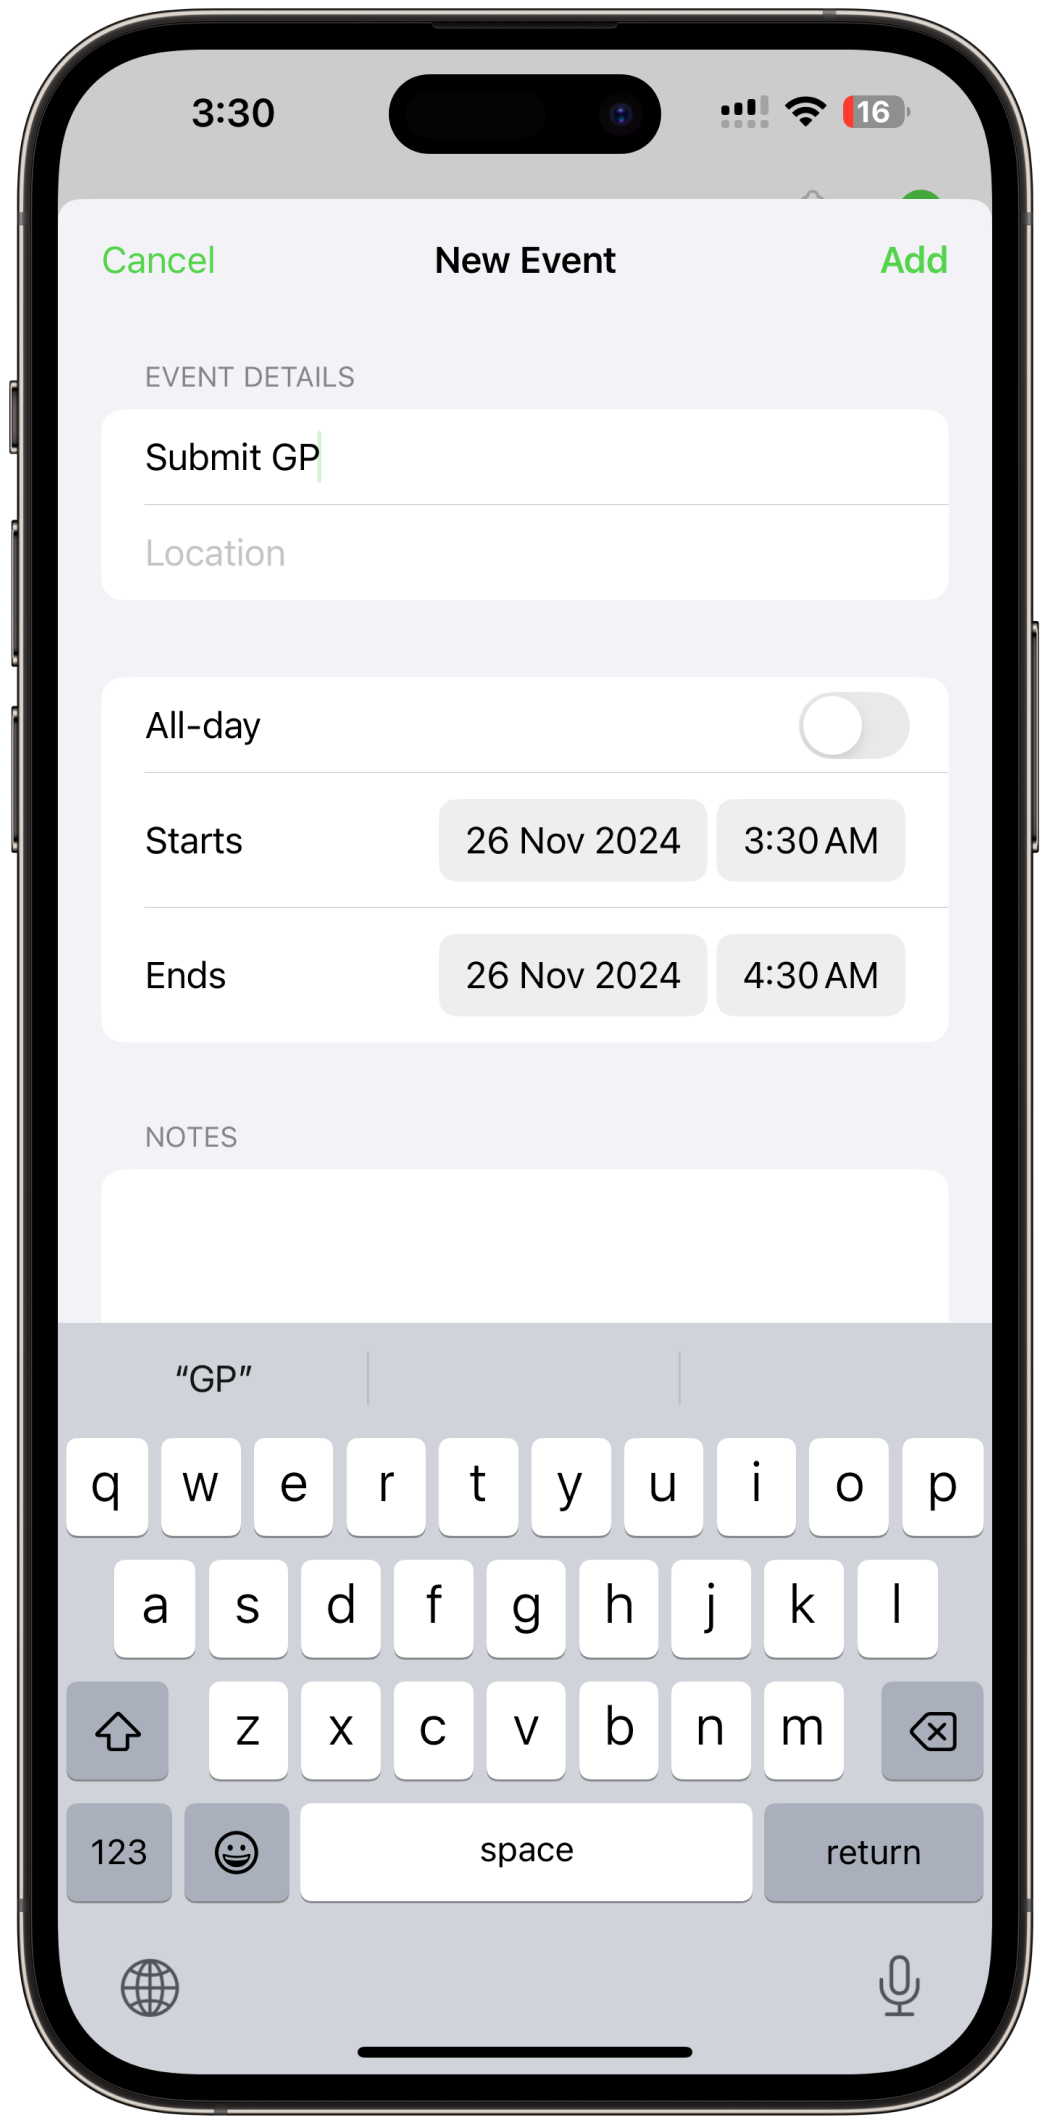
\includegraphics[width=\textwidth]{images/screen6.png}
        \caption{UI Screen 6: Add Event View - All-day}
        \label{fig:ui-screen-6}
    \end{minipage}
\end{figure}

\begin{figure}[!h]
    \begin{minipage}{0.3\textwidth}
        \centering
        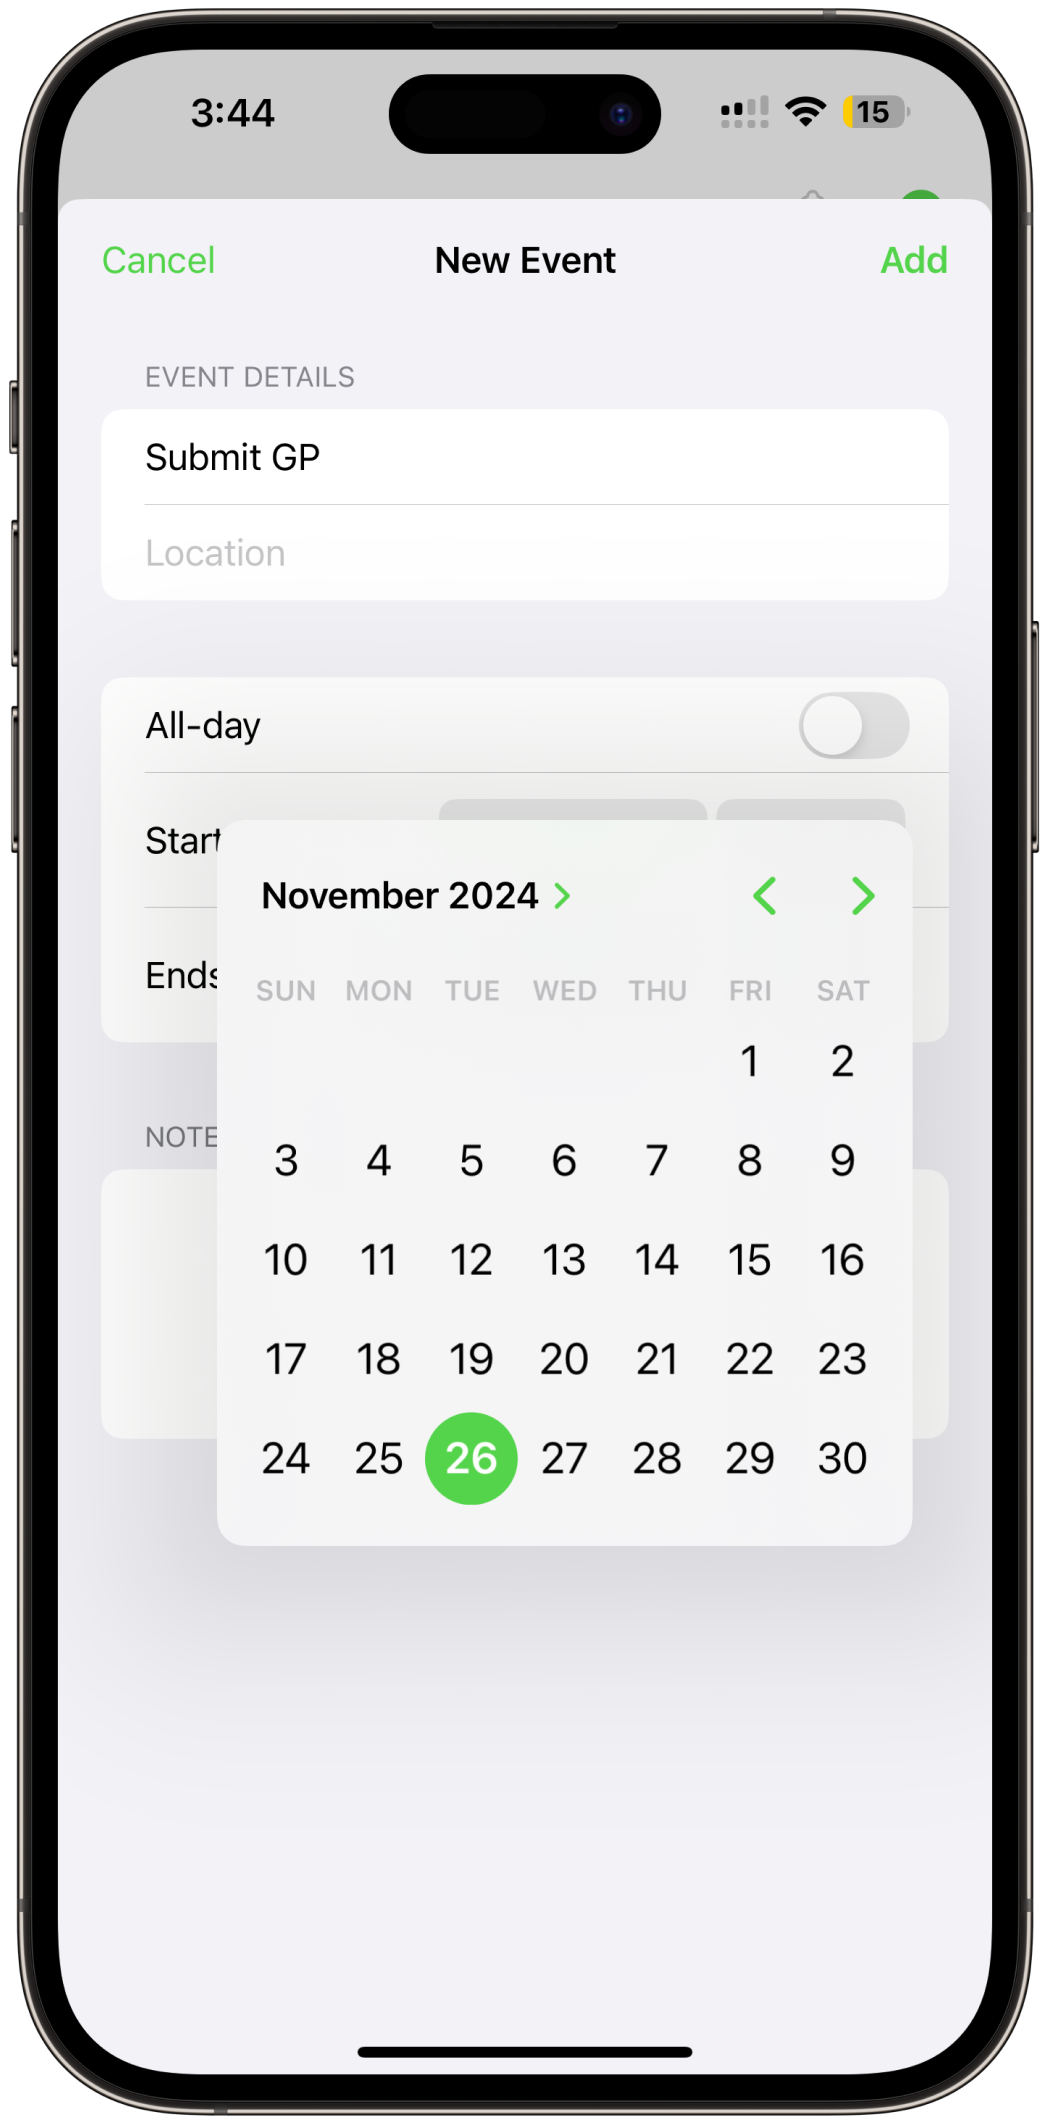
\includegraphics[width=\textwidth]{images/screen7.png}
        \caption{UI Screen 7: Settings View}
        \label{fig:ui-screen-7}
    \end{minipage}
    \hfill
    \begin{minipage}{0.65\textwidth}
        In Figure \ref{fig:ui-screen-7}, the settings page is shown. This pae has the user details, specifcally email, and name. Also the "Connect WhatsApp" button is shown along with the "Connect CalDAV" button. Those two buttons do as they say and allow users to have data sources for the calendar connected. The last button shown is the logout button, and this button is in red to make the user alerted and not click it by mistake. Clicking it will log the user out and take them to the home screen.
    \end{minipage}
\end{figure}

\begin{figure}[!h]
    \begin{minipage}{0.65\textwidth}
        In Figure \ref{fig:ui-screen-8}, the settings page is shown. This pae has the user details, specifcally email, and name. Also the "Connect WhatsApp" button is shown along with the "Connect CalDAV" button. Those two buttons do as they say and allow users to have data sources for the calendar connected. The last button shown is the logout button, and this button is in red to make the user alerted and not click it by mistake. Clicking it will log the user out and take them to the home screen.
    \end{minipage}
    \hfill
    \begin{minipage}{0.3\textwidth}
        \centering
        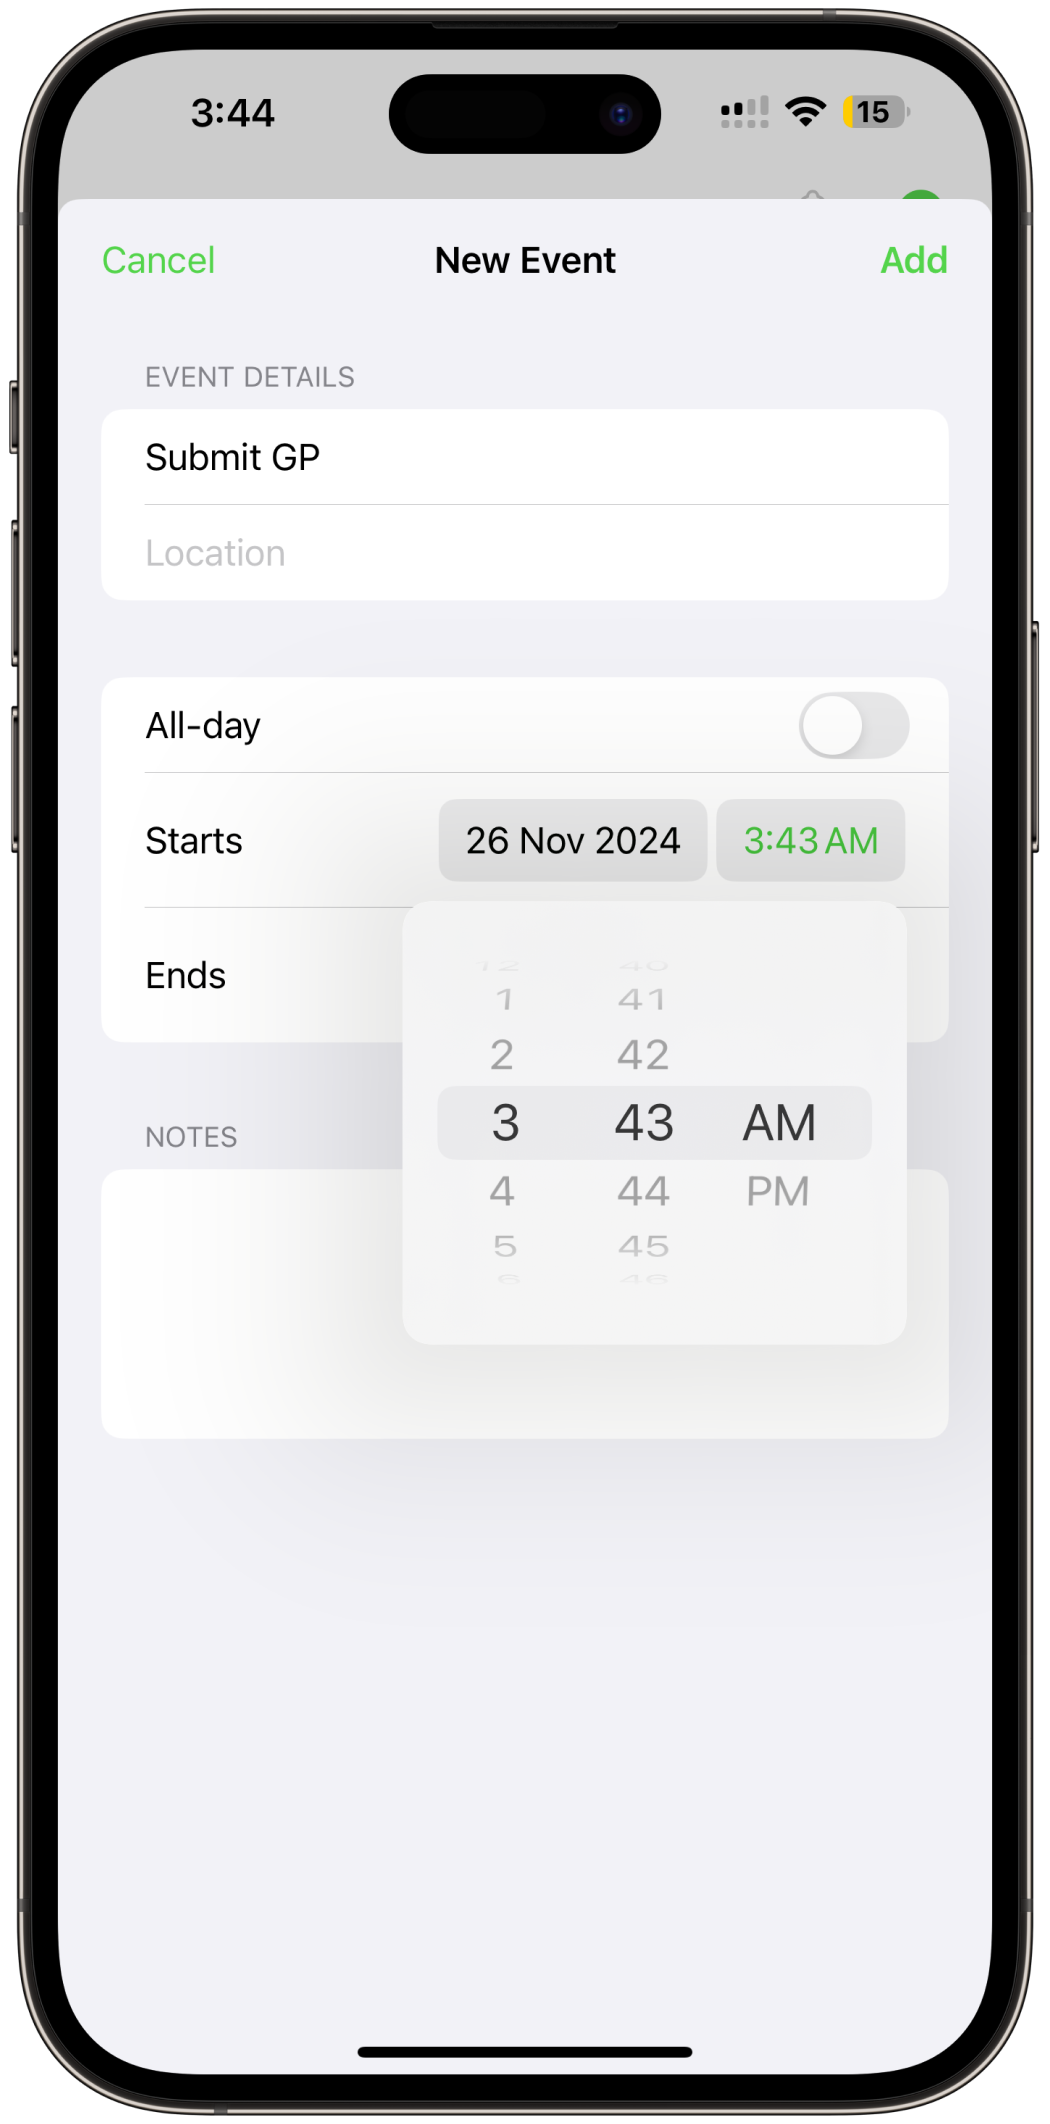
\includegraphics[width=\textwidth]{images/screen8.png}
        \caption{UI Screen 8: Settings View}
        \label{fig:ui-screen-8}
    \end{minipage}
\end{figure}

\begin{figure}[!h]
    \begin{minipage}{0.3\textwidth}
        \centering
        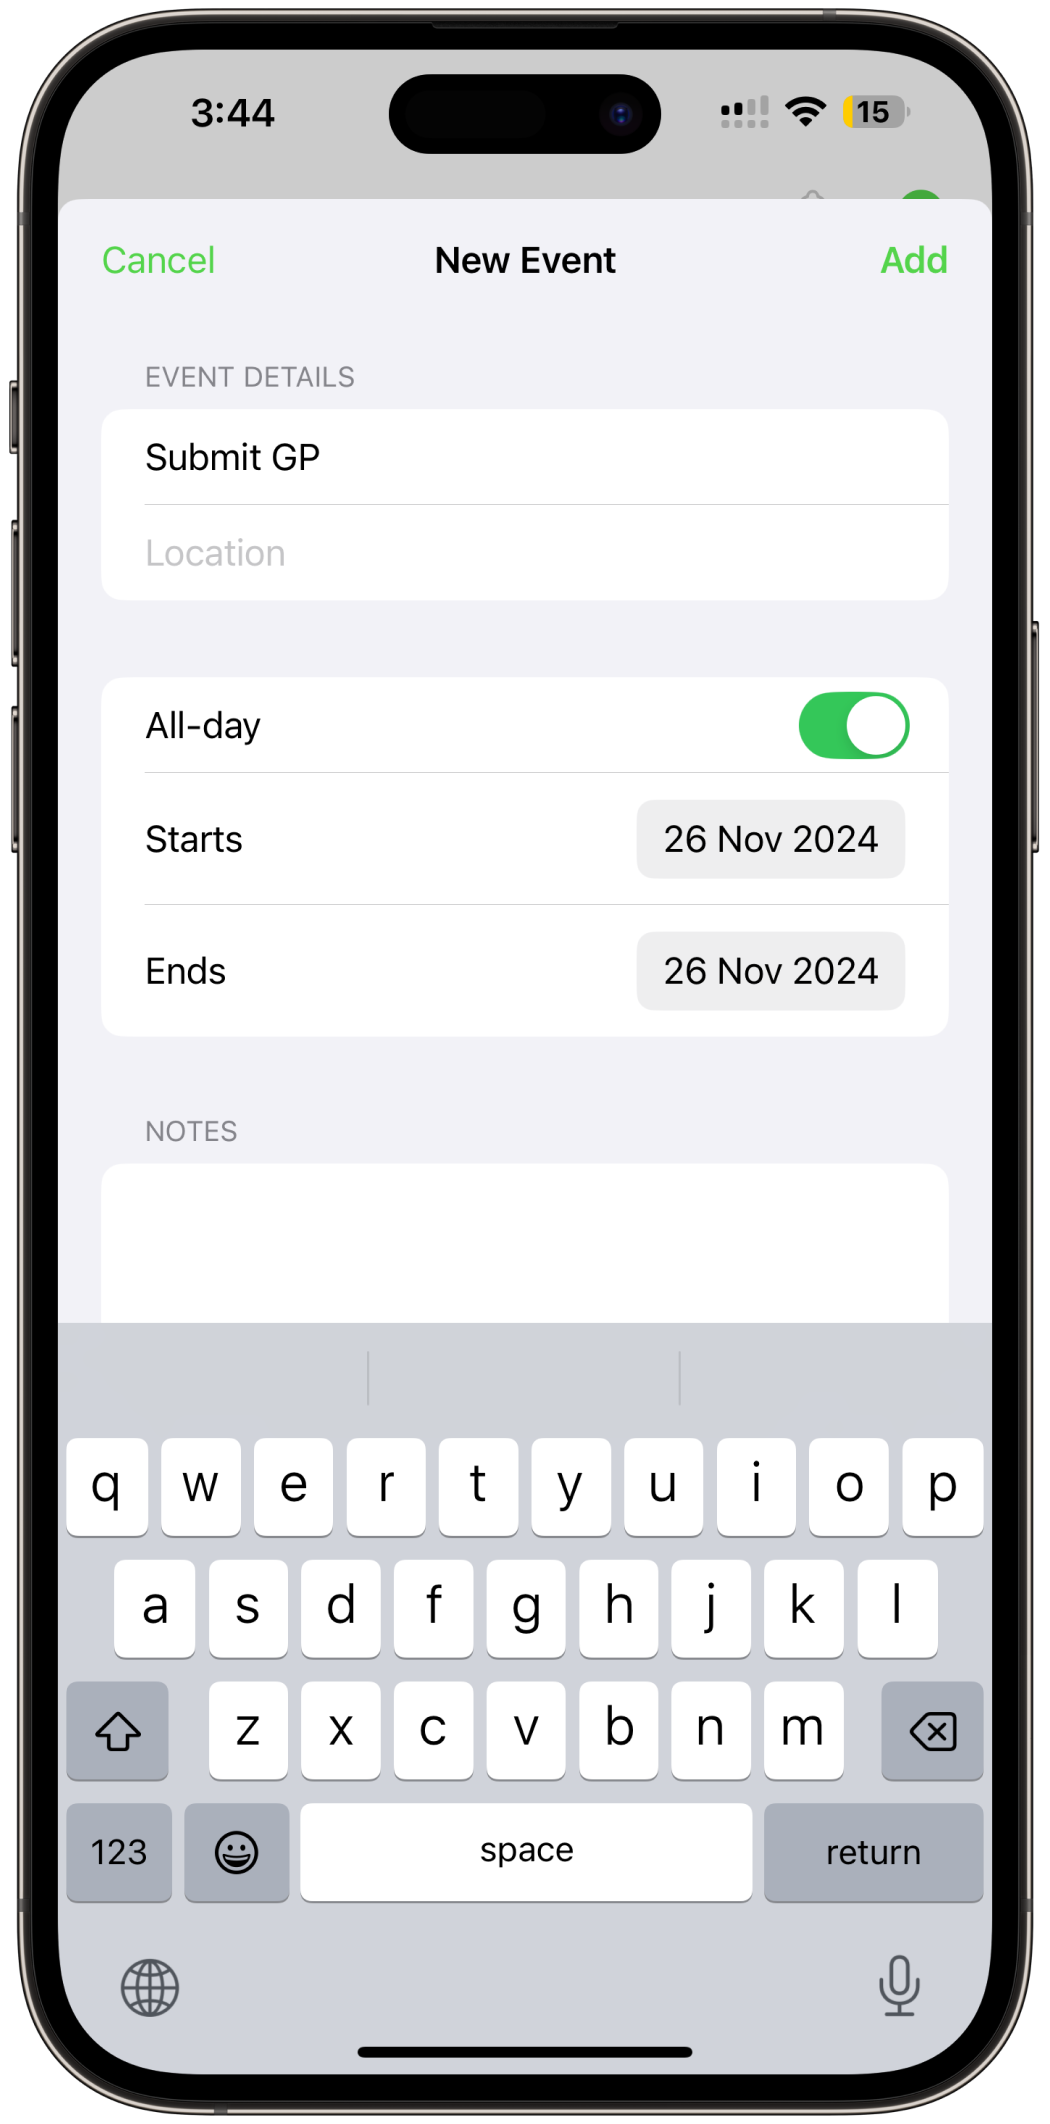
\includegraphics[width=\textwidth]{images/screen9.png}
        \caption{UI Screen 9: Settings View}
        \label{fig:ui-screen-9}
    \end{minipage}
    \hfill
    \begin{minipage}{0.65\textwidth}
        In Figure \ref{fig:ui-screen-9}, the settings page is shown. This pae has the user details, specifcally email, and name. Also the "Connect WhatsApp" button is shown along with the "Connect CalDAV" button. Those two buttons do as they say and allow users to have data sources for the calendar connected. The last button shown is the logout button, and this button is in red to make the user alerted and not click it by mistake. Clicking it will log the user out and take them to the home screen.
    \end{minipage}
\end{figure}

\begin{figure}[!h]
    \begin{minipage}{0.65\textwidth}
        In Figure \ref{fig:ui-screen-10}, the settings page is shown. This pae has the user details, specifcally email, and name. Also the "Connect WhatsApp" button is shown along with the "Connect CalDAV" button. Those two buttons do as they say and allow users to have data sources for the calendar connected. The last button shown is the logout button, and this button is in red to make the user alerted and not click it by mistake. Clicking it will log the user out and take them to the home screen.
    \end{minipage}
    \hfill
    \begin{minipage}{0.3\textwidth}
        \centering
        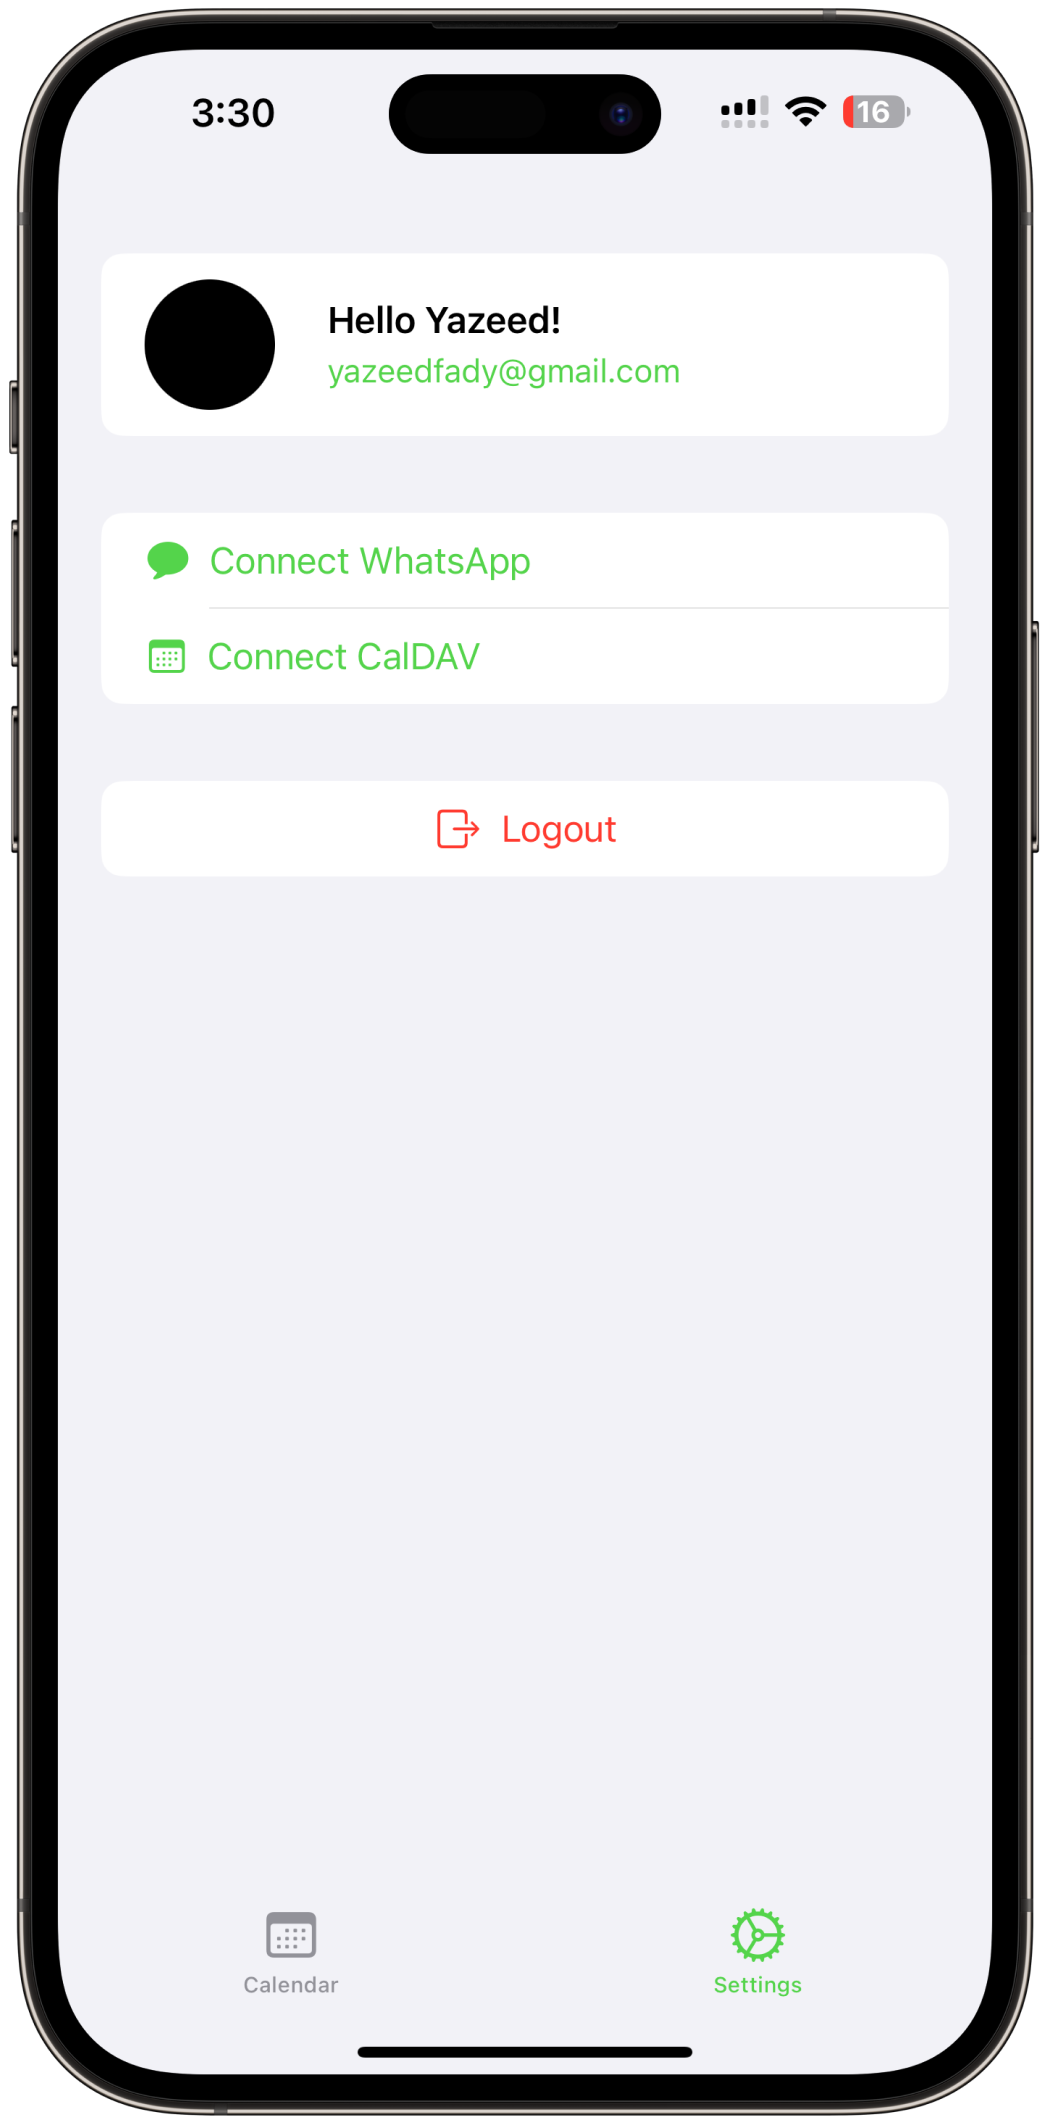
\includegraphics[width=\textwidth]{images/screen10.png}
        \caption{UI Screen 10: Settings View}
        \label{fig:ui-screen-10}
    \end{minipage}
\end{figure}